\documentclass[a4paper,12pt,twoside]{memoir}

% Castellano
\usepackage[spanish,es-tabla]{babel}
\selectlanguage{spanish}\textbf{•}
\usepackage[utf8]{inputenc}
\usepackage[T1]{fontenc}
\usepackage{lmodern} % scalable font
\usepackage{microtype}
\usepackage{placeins}

\RequirePackage{booktabs}
\RequirePackage[table]{xcolor}
\RequirePackage{xtab}
\RequirePackage{multirow}

% Links
\PassOptionsToPackage{hyphens}{url}\usepackage[colorlinks]{hyperref}
\hypersetup{
	allcolors = {red}
}

% Ecuaciones
\usepackage{amsmath}

% Rutas de fichero / paquete
\newcommand{\ruta}[1]{{\sffamily #1}}

% Párrafos
\nonzeroparskip

% Huérfanas y viudas
\widowpenalty100000
\clubpenalty100000

% Evitar solapes en el header
\nouppercaseheads

% Imagenes
\usepackage{graphicx}
\newcommand{\imagen}[2]{
	\begin{figure}[!h]
		\centering
		\includegraphics[width=0.9\textwidth]{#1}
		\caption{#2}\label{fig:#1}
	\end{figure}
	\FloatBarrier
}

\newcommand{\imagenflotante}[2]{
	\begin{figure}%[!h]
		\centering
		\includegraphics[width=0.9\textwidth]{#1}
		\caption{#2}\label{fig:#1}
	\end{figure}
}



% El comando \figura nos permite insertar figuras comodamente, y utilizando
% siempre el mismo formato. Los parametros son:
% 1 -> Porcentaje del ancho de página que ocupará la figura (de 0 a 1)
% 2 --> Fichero de la imagen
% 3 --> Texto a pie de imagen
% 4 --> Etiqueta (label) para referencias
% 5 --> Opciones que queramos pasarle al \includegraphics
% 6 --> Opciones de posicionamiento a pasarle a \begin{figure}
\newcommand{\figuraConPosicion}[6]{%
  \setlength{\anchoFloat}{#1\textwidth}%
  \addtolength{\anchoFloat}{-4\fboxsep}%
  \setlength{\anchoFigura}{\anchoFloat}%
  \begin{figure}[#6]
    \begin{center}%
      \Ovalbox{%
        \begin{minipage}{\anchoFloat}%
          \begin{center}%
            \includegraphics[width=\anchoFigura,#5]{#2}%
            \caption{#3}%
            \label{#4}%
          \end{center}%
        \end{minipage}
      }%
    \end{center}%
  \end{figure}%
}

%
% Comando para incluir imágenes en formato apaisado (sin marco).
\newcommand{\figuraApaisadaSinMarco}[5]{%
  \begin{figure}%
    \begin{center}%
    \includegraphics[angle=90,height=#1\textheight,#5]{#2}%
    \caption{#3}%
    \label{#4}%
    \end{center}%
  \end{figure}%
}
% Para las tablas
\newcommand{\otoprule}{\midrule [\heavyrulewidth]}
%
% Nuevo comando para tablas pequeñas (menos de una página).
\newcommand{\tablaSmall}[5]{%
 \begin{table}
  \begin{center}
   \rowcolors {2}{gray!35}{}
   \begin{tabular}{#2}
    \toprule
    #4
    \otoprule
    #5
    \bottomrule
   \end{tabular}
   \caption{#1}
   \label{tabla:#3}
  \end{center}
 \end{table}
}

%
%Para el float H de tablaSmallSinColores
\usepackage{float}

%
% Nuevo comando para tablas pequeñas (menos de una página).
\newcommand{\tablaSmallSinColores}[5]{%
 \begin{table}[H]
  \begin{center}
   \begin{tabular}{#2}
    \toprule
    #4
    \otoprule
    #5
    \bottomrule
   \end{tabular}
   \caption{#1}
   \label{tabla:#3}
  \end{center}
 \end{table}
}

\newcommand{\tablaApaisadaSmall}[5]{%
\begin{landscape}
  \begin{table}
   \begin{center}
    \rowcolors {2}{gray!35}{}
    \begin{tabular}{#2}
     \toprule
     #4
     \otoprule
     #5
     \bottomrule
    \end{tabular}
    \caption{#1}
    \label{tabla:#3}
   \end{center}
  \end{table}
\end{landscape}
}

%
% Nuevo comando para tablas grandes con cabecera y filas alternas coloreadas en gris.
\newcommand{\tabla}[6]{%
  \begin{center}
    \tablefirsthead{
      \toprule
      #5
      \otoprule
    }
    \tablehead{
      \multicolumn{#3}{l}{\small\sl continúa desde la página anterior}\\
      \toprule
      #5
      \otoprule
    }
    \tabletail{
      \hline
      \multicolumn{#3}{r}{\small\sl continúa en la página siguiente}\\
    }
    \tablelasttail{
      \hline
    }
    \bottomcaption{#1}
    \rowcolors {2}{gray!35}{}
    \begin{xtabular}{#2}
      #6
      \bottomrule
    \end{xtabular}
    \label{tabla:#4}
  \end{center}
}

%
% Nuevo comando para tablas grandes con cabecera.
\newcommand{\tablaSinColores}[6]{%
  \begin{center}
    \tablefirsthead{
      \toprule
      #5
      \otoprule
    }
    \tablehead{
      \multicolumn{#3}{l}{\small\sl continúa desde la página anterior}\\
      \toprule
      #5
      \otoprule
    }
    \tabletail{
      \hline
      \multicolumn{#3}{r}{\small\sl continúa en la página siguiente}\\
    }
    \tablelasttail{
      \hline
    }
    \bottomcaption{#1}
    \begin{xtabular}{#2}
      #6
      \bottomrule
    \end{xtabular}
    \label{tabla:#4}
  \end{center}
}

%
% Nuevo comando para tablas grandes sin cabecera.
\newcommand{\tablaSinCabecera}[5]{%
  \begin{center}
    \tablefirsthead{
      \toprule
    }
    \tablehead{
      \multicolumn{#3}{l}{\small\sl continúa desde la página anterior}\\
      \hline
    }
    \tabletail{
      \hline
      \multicolumn{#3}{r}{\small\sl continúa en la página siguiente}\\
    }
    \tablelasttail{
      \hline
    }
    \bottomcaption{#1}
  \begin{xtabular}{#2}
    #5
   \bottomrule
  \end{xtabular}
  \label{tabla:#4}
  \end{center}
}



\definecolor{cgoLight}{HTML}{EEEEEE}
\definecolor{cgoExtralight}{HTML}{FFFFFF}

%
% Nuevo comando para tablas grandes sin cabecera.
\newcommand{\tablaSinCabeceraConBandas}[5]{%
  \begin{center}
    \tablefirsthead{
      \toprule
    }
    \tablehead{
      \multicolumn{#3}{l}{\small\sl continúa desde la página anterior}\\
      \hline
    }
    \tabletail{
      \hline
      \multicolumn{#3}{r}{\small\sl continúa en la página siguiente}\\
    }
    \tablelasttail{
      \hline
    }
    \bottomcaption{#1}
    \rowcolors[]{1}{cgoExtralight}{cgoLight}

  \begin{xtabular}{#2}
    #5
   \bottomrule
  \end{xtabular}
  \label{tabla:#4}
  \end{center}
}




\graphicspath{ {./img/} }

% Capítulos
\chapterstyle{bianchi}
\newcommand{\capitulo}[2]{
	\setcounter{chapter}{#1}
	\setcounter{section}{0}
	\chapter*{#2}
	\addcontentsline{toc}{chapter}{#2}
	\markboth{#2}{#2}
}

% Apéndices
\renewcommand{\appendixname}{Apéndice}
\renewcommand*\cftappendixname{\appendixname}

\newcommand{\apendice}[1]{
	%\renewcommand{\thechapter}{A}
	\chapter{#1}
}

\renewcommand*\cftappendixname{\appendixname\ }

% Formato de portada
\makeatletter
\usepackage{xcolor}
\newcommand{\tutor}[1]{\def\@tutor{#1}}
\newcommand{\course}[1]{\def\@course{#1}}
\definecolor{cpardoBox}{HTML}{E6E6FF}
\def\maketitle{
  \null
  \thispagestyle{empty}
  % Cabecera ----------------
\noindent
\includegraphics[width=\textwidth]{cabecera}\vspace{1cm}%
  \vfill
  % Título proyecto y escudo informática ----------------
  \colorbox{cpardoBox}{%
    \begin{minipage}{.8\textwidth}
      \vspace{.5cm}\Large
      \begin{center}
      \textbf{TFG del Grado en Ingeniería Informática}\vspace{.6cm}\\
      \textbf{\LARGE\@title{}}
      \end{center}
      \vspace{.2cm}
    \end{minipage}

  }%
  \hfill\begin{minipage}{.20\textwidth}
    
\includegraphics[width=\textwidth]{escudoInfor}
  \end{minipage}
  \vfill
  % Datos de alumno, curso y tutores ------------------
  \begin{center}%
  {%
    \noindent\LARGE
    Presentado por \@author{}\\ 
    en Universidad de Burgos --- \@date{}\\
    Tutor: \@tutor{}\\
  }%
  \end{center}%
  \null
  \cleardoublepage
  }
\makeatother


% Datos de portada
\title{título del TFG \\Documentación Técnica}
\author{nombre alumno}
\tutor{nombre tutor}
\date{\today}

\begin{document}

\maketitle



\cleardoublepage



%%%%%%%%%%%%%%%%%%%%%%%%%%%%%%%%%%%%%%%%%%%%%%%%%%%%%%%%%%%%%%%%%%%%%%%%%%%%%%%%%%%%%%%%



\frontmatter


\clearpage

% Indices
\tableofcontents

\clearpage

\listoffigures

\clearpage

\listoftables

\clearpage

\mainmatter

\appendix

\apendice{Plan de Proyecto Software}

\section{Introducción}

\section{Planificación temporal}

\section{Estudio de viabilidad}

\subsection{Viabilidad económica}

\subsection{Viabilidad legal}



\apendice{Especificación de Requisitos} \label{requisitos}

\section{Introducción}

En este anexo se detallan los objetivos del proyecto y los requisitos que debe cumplir el \textit{software} desarrollado. Estos requisitos se han indicado al inicio del proyecto, pero a lo largo de su desarrollo se han ido añadiendo otros adicionales, por lo que aquí se recogen y explican todos adecuadamente. Parcialmente, se han seguido indicaciones del estándar IEEE 830-1998 para la especificación de requisitos.

\section{Objetivos generales}

Los objetivos que se pretenden alcanzar en este proyecto son los siguientes:

\begin{itemize}
\tightlist
	\item Desarrollar un videojuego de carreras para PC, compatible con Windows y Linux.
	\item Ofrecer una buena jugabilidad y accesibilidad al usuario, con una curva de aprendizaje sencilla.
	\item Aprender a usar Unity, sus funcionalidades y la programación en el lenguaje que le corresponde.
	\item Asentar unas bases para proyectos similares.
\end{itemize}

\section{Catalogo de requisitos}

En este apartado se detallan los requisitos funcionales y no funcionales de la aplicación desarrollada.

\subsection{Requisitos funcionales}
\begin{itemize}
\tightlist
\item 
	\textbf{RF-1 Jugar:} La aplicación debe permitir iniciar una partida.
	
	\begin{itemize}
    \tightlist
    \item
      	\textbf{RF-1.1 Seleccionar modo:} El usuario debe poder escoger entre los modos de juego disponibles.
      	
      	\begin{itemize}
		\tightlist
		\item
			\textbf{RF-1.1.1 Partida contrarreloj:} La aplicación debe poder crear una partida de carrera a contrarreloj.			
			\begin{itemize}
			\tightlist
				\item \textbf{RF-1.1.1.1 Conteo de vueltas}: En la partida debe haber un contador de vueltas que indique el número de vuelta en el que se ubica el usuario, así como el número total de vueltas a realizar.
				\item \textbf{RF-1.1.1.2 Cronómetro de tiempo:}: En la partida debe haber un cronómetro que cuente el tiempo realizado en una vuelta. Este cronómetro debe ponerse a cero cada vez que, habiendo atravesado todos los puntos de control previamente, se atraviese la línea de meta.
				\item \textbf{RF-1.1.1.3 Indicador de mejor tiempo:} Cada mejor tiempo realizado al completar una vuelta debe ser actualizado en un letrero. En caso de no realizarse un tiempo mejor, se dejará con el último mejor tiempo. Cada vez que se empiece una nueva partida debe estar restaurado a 0.
			\end{itemize}
    	
    	\end{itemize}
    	\item
    		\textbf{RF-1.2 Seleccionar personaje:} El usuario debe poder escoger entre las diferentes personajes disponibles para jugar.
		\item    	
    		\textbf{RF-1.3 Seleccionar circuito:} El usuario debe poder escoger entre los diferentes escenarios disponibles en los que realizar la carrera.
    	\item
    		\textbf{RF-1.4 Conducir vehículo:} El usuario debe poder conducir un vehículo escogido previamente.
    		\begin{itemize}
			\tightlist
				\item \textbf{RF-1.4.1 Aceleración del vehículo:} El vehículo debe poder acelerar a petición del usuario. Debe poder combinarse en su uso simultáneo con el giro.
				\item \textbf{RF-1.4.2 Deceleración del vehículo:} El vehículo debe poder decelerar e ir en dirección marcha atrás a petición del usuario. Debe poder combinarse en su uso simultáneo con el giro.
				\item \textbf{RF-1.4.3 Giro del vehículo:} El vehículo debe poder girar hacia el lado izquierdo o hacia el lado derecho a petición del usuario. Debe poder combinarse en su uso simultáneo con la aceleración o la deceleración.
				\item \textbf{RF-1.4.4 Recolocación del vehículo:} El vehículo debe poder ser recolocado manualmente en un punto de control previo a petición del usuario. En caso de caer al vacío, debe poder ser recolocado automáticamente.
			\end{itemize}
    \end{itemize}
    
	\item \textbf{RF-2 Instrucciones:} La aplicación debe ofrecer al usuario la posibilidad de consultar unas instrucciones de juego para 
	\item \textbf{RF-3 Créditos:} La aplicación ha de ofrecer la posibilidad de conocer al usuario quiénes han realizado la aplicación en los distintos aspectos que la componen.
	\item \textbf{RF-4 Salir:} El usuario debe poder salir de la aplicación mediante una opción ofrecida por la misma.
	\begin{itemize}
	\tightlist
		\item \textbf{RF-4.1 Salir de la partida:} El usuario debe poder salir de la partida en curso mediante una opción en el menú.
	\end{itemize}
	\item \textbf{RF-5 Volver a la pantalla anterior:} La aplicación debe ofrecer la posibilidad de volver a la pantalla anterior al menú en el que se encuentra el usuario.
	\item \textbf{RF-6 Pausar partida:} La aplicación debe ofrecer la posibilidad de pausar la partida a petición del usuario, así como continuarla una vez pausada.
\end{itemize}

\subsection{Requisitos no funcionales}

Estos requisitos se han obtenido en base a las características el estándar internacional para la evaluación de la calidad del software.

\begin{itemize}
\tightlist
\item 
	\textbf{RNF-1 Usabilidad:} La aplicación debe ser sencilla de jugar y divertida. La curva de aprendizaje ha de ser baja para que el usuario no desista en comprender el funcionamiento y mejorar, a la vez que tiene que ser capaz de divertirse gracias a las mecánicas del videojuego. Por ello, la interfaz es \"amigable\" de cara al usuario.

\item 
	\textbf{RNF-2 Eficiencia:} La aplicación debe poder ser ejecutada en computadoras de gama media, con tiempos de carga entre pantallas aceptables y una jugabilidad fluida sin ralentizaciones de \textit{frames}. Además, debe poderse incrementar los recursos de los que dispone la aplicación realizando distintas mejoras que impliquen una mayor eficiencia.
	
\item 
	\textbf{RNF-3 Multiplataforma:} La aplicación debe poder ser distribuida para sistemas operativos Windows y Linux, con su correspondiente correcta ejecución en los mismos. 
	
\item 
	\textbf{RNF-4 Facilidad de mantenimiento:} Tiene que asegurar la posibilidad de ser extensible (pudiendo añadir funcionalidades nuevas al videojuego), modificable y corregible de manera sencilla.

\item 
	\textbf{RNF-5 Portabilidad:} Debe ser fácilmente transferible y adaptable a nuevas plataformas de juego.

\end{itemize}
\section{Especificación de requisitos}

En esta sección se muestra el diagrama de casos de uso de la aplicación, así como el desglose de cada uno de esos casos.

\subsection{Diagrama de casos de uso}

El diagrama de casos de uso corresponde al siguiente mostrado:

\imagen{use-case-diagram}{Diagrama de casos de uso}

\subsection{Actores}

El número de actores que interactúan con este sistema es de uno, siendo el usuario que lo utiliza el único actor.

\subsection{Casos de uso}

\begin{longtable}{>{\raggedright}b{0.2\linewidth}>{\raggedright\arraybackslash}b{0.7\linewidth}}

	\toprule
	\textbf{CU-01} & \textbf{Jugar} \\
	\toprule
	\endhead

	\toprule
	\caption{CU-01 Jugar}
	\endfoot
	
	\small{\textbf{Descripción}} & Jugar una partida. \\
	\small{\textbf{Autor}} & Alejandro Goicoechea Román \\
	\small{\textbf{Requisitos}} & RF-1 \\
	\small{\textbf{relacionados}} & \\
	\small{\textbf{Precondición}} & Tener el videojuego iniciado. \\
	\small{\textbf{Acciones}} & \quad {\small 1. Si no lo ha realizado previamente, el usuario ejecuta} \\
	& \quad {\small la aplicación.} \\
	& \quad {\small 2. El usuario pulsa en el botón de ``Jugar'' en el menú} \\
	& \quad {\small principal.} \\
	\small{\textbf{Postcondición}} & Se muestra la pantalla de selección de modo de juego. \\
	\small{\textbf{Excepciones}} & - \\
	\small{\textbf{Importancia}} & Alta. \\
	
\end{longtable}

\begin{longtable}{>{\raggedright}b{0.2\linewidth}>{\raggedright\arraybackslash}b{0.7\linewidth}}

	\toprule
	\textbf{CU-02} & \textbf{Seleccionar modo} \\
	\toprule
	\endhead

	\toprule
	\caption{CU-02 Seleccionar modo}
	\endfoot
	
	\small{\textbf{Descripción}} & Escoger entre los diferentes modos de juego \\ 
	&  disponibles. \\
	\small{\textbf{Autor}} & Alejandro Goicoechea Román \\
	\small{\textbf{Requisitos}} & RF-1, RF-1.1 \\
	\small{\textbf{relacionados}} & \\
	\small{\textbf{Precondición}} & Haber seleccionado la opción de "Jugar". \\
	\small{\textbf{Acciones}} & \quad {\small 1. Pulsar en el modo de juego deseado.} \\
	\small{\textbf{Postcondición}} & Se muestra la pantalla de selección de personaje. \\
	\small{\textbf{Excepciones}} & - \\
	\small{\textbf{Importancia}} & Alta. \\
	
\end{longtable}

\begin{longtable}{>{\raggedright}b{0.2\linewidth}>{\raggedright\arraybackslash}b{0.7\linewidth}}

	\toprule
	\textbf{CU-03} & \textbf{Seleccionar personaje} \\
	\toprule
	\endhead

	\toprule
	\caption{CU-03 Seleccionar personaje}
	\endfoot
	
	\small{\textbf{Descripción}} & Escoger un personaje de entre todos los personajes \\
	&  disponibles para conducir con él. \\
	\small{\textbf{Autor}} & Alejandro Goicoechea Román \\
	\small{\textbf{Requisitos}} & RF-1, RF-1.1.1, RF-1.2 \\
	\small{\textbf{relacionados}} & \\
	\small{\textbf{Precondición}} & Haber escogido un modo de juego. \\
	\small{\textbf{Acciones}} & \quad {\small 1. Pulsar en un icono de personaje.} \\
	\small{\textbf{Postcondición}} & Se muestra la pantalla de selección de circuito. \\
	\small{\textbf{Excepciones}} & - \\
	\small{\textbf{Importancia}} & Alta. \\
	
\end{longtable}

\begin{longtable}{>{\raggedright}b{0.2\linewidth}>{\raggedright\arraybackslash}b{0.7\linewidth}}

	\toprule
	\textbf{CU-04} & \textbf{Seleccionar circuito} \\
	\toprule
	\endhead

	\toprule
	\caption{CU-04 Seleccionar circuito}
	\endfoot
	
	\small{\textbf{Descripción}} & Seleccionar un circuito de entre todos los disponibles \\
	& para recorrerlo. \\
	&  \\
	\small{\textbf{Autor}} & Alejandro Goicoechea Román \\
	\small{\textbf{Requisitos}} & RF-1, RF-1.1.1, RF 1.2, RF-1.3 \\
	\small{\textbf{relacionados}} & \\
	\small{\textbf{Precondición}} & Haber seleccionado un personaje. \\
	\small{\textbf{Acciones}} & \quad {\small 1. Pulsar en un icono de circuito. } \\
	\small{\textbf{Postcondición}} & Empieza la partida con las opciones previas \\ 
	& seleccionadas. \\
	\small{\textbf{Excepciones}} & - \\
	\small{\textbf{Importancia}} & Alta. \\
	
\end{longtable}

\begin{longtable}{>{\raggedright}b{0.2\linewidth}>{\raggedright\arraybackslash}b{0.7\linewidth}}

	\toprule
	\textbf{CU-05} & \textbf{Conducir vehículo} \\
	\toprule
	\endhead

	\toprule
	\caption{CU-05 Conducir vehículo}
	\endfoot
	
	\small{\textbf{Descripción}} & Conducir el vehículo escogido por el usuario. \\
	\small{\textbf{Autor}} & Alejandro Goicoechea Román \\
	\small{\textbf{Requisitos}} & RF-1, RF-1.4, RF-1.4.1, RF-1.4.2, RF-1.4.3 \\
	\small{\textbf{relacionados}} & \\
	\small{\textbf{Precondición}} & Haber comenzado una partida. \\
	\small{\textbf{Acciones}} & \quad {\small 1. El usuario pulsa cualquiera de las acciones } \\
	& \quad {\small asociadas a la conducción del vehículo. } \\
	\small{\textbf{Postcondición}} & El vehículo debe moverse en base a la acción \\
	& realizada. \\
	\small{\textbf{Excepciones}} & - \\
	\small{\textbf{Importancia}} & Alta. \\
	
\end{longtable}

\begin{longtable}{>{\raggedright}b{0.2\linewidth}>{\raggedright\arraybackslash}b{0.7\linewidth}}

	\toprule
	\textbf{CU-06} & \textbf{Acelerar vehículo} \\
	\toprule
	\endhead

	\toprule
	\caption{CU-06 Acelerar vehículo}
	\endfoot
	
	\small{\textbf{Descripción}} & Acelerar el vehículo durante el tiempo que desea el \\
	& usuario.  \\
	\small{\textbf{Autor}} & Alejandro Goicoechea Román \\
	\small{\textbf{Requisitos}} & RF-1, RF-1.4, RF-1.4.1, RF-1.4.3 \\
	\small{\textbf{relacionados}} & \\
	\small{\textbf{Precondición}} & Haber comenzado una partida. \\
	\small{\textbf{Acciones}} & \quad {\small 1. El usuario pulsa la tecla "W" o la tecla de ``flecha } \\
	& \quad {\small arriba'' de manera intermitente o constante. } \\
	& \quad {\small 2. De manera opcional, el usuario pulsa, combinando } \\
	& \quad {\small con la tecla de aceleración, las teclas de giro} \\
	& \quad {\small (``A''/``flecha izquierda'' o ``D''/``flecha derecha''). } \\
	\small{\textbf{Postcondición}} & El vehículo se desplaza hacia \\
	& adelante o hacia adelante con giro según lo pulsado previamente. \\
	\small{\textbf{Excepciones}} & - \\
	\small{\textbf{Importancia}} & Muy alta. \\
	
\end{longtable}

\begin{longtable}{>{\raggedright}b{0.2\linewidth}>{\raggedright\arraybackslash}b{0.7\linewidth}}

	\toprule
	\textbf{CU-07} & \textbf{Decelerar vehículo} \\
	\toprule
	\endhead

	\toprule
	\caption{CU-07 Decelerar vehículo}
	\endfoot
	
	\small{\textbf{Descripción}} & Decelerar el vehículo durante el tiempo que desea el \\
	& usuario.  \\
	\small{\textbf{Autor}} & Alejandro Goicoechea Román \\
	\small{\textbf{Requisitos}} & RF-1, RF-1.4, RF-1.4.2, RF-1.4.3 \\
	\small{\textbf{relacionados}} & \\
	\small{\textbf{Precondición}} & Haber comenzado una partida. \\
	\small{\textbf{Acciones}} & \quad {\small 1. El usuario pulsa la tecla "S" o la tecla de ``flecha } \\
	& \quad {\small abajo'' de manera intermitente o constante. } \\
	& \quad {\small 2. De manera opcional, el usuario pulsa, combinando } \\
	& \quad {\small con la tecla de deceleración, las teclas de giro} \\
	& \quad {\small (``A''/``flecha izquierda'' o ``D''/``flecha derecha''). } \\
	\small{\textbf{Postcondición}} & El vehículo se desplaza hacia atrás o hacia atrás \\
	&  con giro según lo pulsado previamente. Si el vehículo está en movimiento, el vehículo decelera. \\
	\small{\textbf{Excepciones}} & - \\
	\small{\textbf{Importancia}} & Muy alta. \\
	
\end{longtable}

\begin{longtable}{>{\raggedright}b{0.2\linewidth}>{\raggedright\arraybackslash}b{0.7\linewidth}}

	\toprule
	\textbf{CU-08} & \textbf{Girar vehículo} \\
	\toprule
	\endhead

	\toprule
	\caption{CU-08 Girar vehículo}
	\endfoot
	
	\small{\textbf{Descripción}} & Girar vehículo sobre sí mismo si está parado o hacia \\
	& el lado deseado en estado de movimiento. \\
	\small{\textbf{Autor}} & Alejandro Goicoechea Román \\
	\small{\textbf{Requisitos}} & RF-1, RF-1.4, RF-1.4.1, RF-1.4.2, RF-1.4.3 \\
	\small{\textbf{relacionados}} & \\
	\small{\textbf{Precondición}} & Haber comenzado una partida. \\
	\small{\textbf{Acciones}} & \quad {\small 1. El usuario pulsa la tecla de giro a la izquierda} \\
	& \quad {\small (``A''/``flecha izquierda'') o la tecla de giro a la} \\
	& \quad {\small derecha (``D''/``flecha derecha'') mientras el vehículo} \\
	& \quad {\small está en movimiento o mientras el vehículo está en} \\
	& \quad {\small estado de reposo. } \\
	\small{\textbf{Postcondición}} & El vehículo gira en la dirección indicada. \\
	\small{\textbf{Excepciones}} & - \\
	\small{\textbf{Importancia}} & Muy alta. \\
	
\end{longtable}

\begin{longtable}{>{\raggedright}b{0.2\linewidth}>{\raggedright\arraybackslash}b{0.7\linewidth}}

	\toprule
	\textbf{CU-09} & \textbf{Recolocar vehículo} \\
	\toprule
	\endhead

	\toprule
	\caption{CU-09 Recolocar vehículo}
	\endfoot
	
	\small{\textbf{Descripción}} & Permite recolocar el vehículo manualmente en el \\
	& último punto de control atravesado. \\
	\small{\textbf{Autor}} & Alejandro Goicoechea Román \\
	\small{\textbf{Requisitos}} & RF-1, RF-1.4, RF-1.4.4 \\
	\small{\textbf{relacionados}} &  \\
	\small{\textbf{Precondición}} & Haber comenzado una partida. \\
	\small{\textbf{Acciones}} & \quad {\small 1. Pulsar la tecla ``R'' para recolocar el vehículo. } \\
	\small{\textbf{Postcondición}} & El vehículo se recoloca en el punto de control \\
	& previamente atravesado. \\
	\small{\textbf{Excepciones}} & - \\
	\small{\textbf{Importancia}} & Alta. \\
	
\end{longtable}

\begin{longtable}{>{\raggedright}b{0.2\linewidth}>{\raggedright\arraybackslash}b{0.7\linewidth}}

	\toprule
	\textbf{CU-10} & \textbf{Partida contrarreloj} \\
	\toprule
	\endhead

	\toprule
	\caption{CU-10 Partida contrarreloj}
	\endfoot
	
	\small{\textbf{Descripción}} & Jugar una partida contrarreloj con todos los \\
	& elementos que conforman ese modo de juego. \\
	\small{\textbf{Autor}} & Alejandro Goicoechea Román \\
	\small{\textbf{Requisitos}} & RF-1, RF-1.1.1, RF-1.2, RF-1.3, RF-1.4 \\
	\small{\textbf{relacionados}} & \\
	\small{\textbf{Precondición}} & Haber seleccionado este modo de juego. \\
	\small{\textbf{Acciones}} & \quad {\small 1. Jugar la partida siguiendo las intrucciones previas} \\
	& \quad {\small vistas.} \\
	\small{\textbf{Postcondición}} & La partida se comporta como un juego de carreras \\
	& contrarreloj. \\
	\small{\textbf{Excepciones}} & - \\
	\small{\textbf{Importancia}} & Alta. \\
	
\end{longtable}

\begin{longtable}{>{\raggedright}b{0.2\linewidth}>{\raggedright\arraybackslash}b{0.7\linewidth}}

	\toprule
	\textbf{CU-11} & \textbf{Conteo de vueltas} \\
	\toprule
	\endhead

	\toprule
	\caption{CU-11 Conteo de vueltas}
	\endfoot
	
	\small{\textbf{Descripción}} & Contar las vueltas que realiza el usuario, así como el \\
	& número total a realizar. \\
	\small{\textbf{Autor}} & Alejandro Goicoechea Román \\
	\small{\textbf{Requisitos}} & RF-1, RF-1.1.1, RF-1.1.1.1 \\
	\small{\textbf{relacionados}} & \\
	\small{\textbf{Precondición}} & Haber comenzado una partida. \\
	\small{\textbf{Acciones}} & \quad {\small 1. Se muestran las vueltas a realizar. } \\
	& \quad {\small 2. Se muestran las vueltas en la que se encuentra el} \\
	& \quad {\small usuario.} \\
	& \quad {\small 3. Por cada vuelta que realice el usuario, el contador} \\
	& \quad {\small actualizará el número de vueltas sumando una a } \\
	& \quad {\small éstas. } \\
	\small{\textbf{Postcondición}} & El contador se actualiza sumando nuevas vueltas. \\
	\small{\textbf{Excepciones}} & - \\
	\small{\textbf{Importancia}} & Alta. \\
	
\end{longtable}

\begin{longtable}{>{\raggedright}b{0.2\linewidth}>{\raggedright\arraybackslash}b{0.7\linewidth}}

	\toprule
	\textbf{CU-12} & \textbf{Cronómetro de tiempo} \\
	\toprule
	\endhead

	\toprule
	\caption{CU-12 Cronómetro de tiempo}
	\endfoot
	
	\small{\textbf{Descripción}} & Contar el tiempo por vuelta realizada. \\
	\small{\textbf{Autor}} & Alejandro Goicoechea Román \\
	\small{\textbf{Requisitos}} & RF-1, RF-1.1.1, RF-1.1.1.2 \\
	\small{\textbf{relacionados}} & \\
	\small{\textbf{Precondición}} & Haber comenzado una partida. \\
	\small{\textbf{Acciones}} & \quad {\small 1. El cronómetro cuenta el tiempo por vuelta} \\
	& \quad {\small  realizada. } \\
	& \quad {\small 2. Por cada vuelta realizada, se restaura a 0. } \\
	\small{\textbf{Postcondición}} & Muestra el tiempo correctamente. \\
	\small{\textbf{Excepciones}} & - \\
	\small{\textbf{Importancia}} & Alta. \\
	
\end{longtable}

\begin{longtable}{>{\raggedright}b{0.2\linewidth}>{\raggedright\arraybackslash}b{0.7\linewidth}}

	\toprule
	\textbf{CU-13} & \textbf{Indicador de mejor tiempo} \\
	\toprule
	\endhead

	\toprule
	\caption{CU-13 Indicador de mejor tiempo}
	\endfoot
	
	\small{\textbf{Descripción}} & Indicar el mejor tiempo de vuelta realizada. \\
	\small{\textbf{Autor}} & Alejandro Goicoechea Román \\
	\small{\textbf{Requisitos}} & RF-1, RF-1.1.1, RF-1.1.1.3 \\
	\small{\textbf{relacionados}} & \\
	\small{\textbf{Precondición}} & Haber comenzado una partida. \\
	\small{\textbf{Acciones}} & \quad {\small 1. Por cada vuelta completada, si el tiempo es mejor } \\
	& \quad {\small al previo indicado, el contador se actualiza. } \\
	& \quad {\small } \\
	\small{\textbf{Postcondición}} & Muestra el mejor tiempo realizado. \\
	\small{\textbf{Excepciones}} & - \\
	\small{\textbf{Importancia}} & Alta. \\
	
\end{longtable}

\begin{longtable}{>{\raggedright}b{0.2\linewidth}>{\raggedright\arraybackslash}b{0.7\linewidth}}

	\toprule
	\textbf{CU-14} & \textbf{Instrucciones} \\
	\toprule
	\endhead

	\toprule
	\caption{CU-14 Instrucciones}
	\endfoot
	
	\small{\textbf{Descripción}} & Visualizar las intrucciones de juego. \\
	\small{\textbf{Autor}} & Alejandro Goicoechea Román \\
	\small{\textbf{Requisitos}} & RF-2 \\
	\small{\textbf{relacionados}} & \\
	\small{\textbf{Precondición}} & Encontrarse en el menú principal. \\
	\small{\textbf{Acciones}} & \quad {\small 1. Pulsar en el botón de instrucciones. } \\
	\small{\textbf{Postcondición}} & Se visualizan las instrucciones del juego. \\
	\small{\textbf{Excepciones}} & - \\
	\small{\textbf{Importancia}} & Alta. \\
	
\end{longtable}

\begin{longtable}{>{\raggedright}b{0.2\linewidth}>{\raggedright\arraybackslash}b{0.7\linewidth}}

	\toprule
	\textbf{CU-15} & \textbf{Créditos} \\
	\toprule
	\endhead

	\toprule
	\caption{CU-15 Créditos}
	\endfoot
	
	\small{\textbf{Descripción}} & Visualizar los créditos del juego con los participantes \\
	& involucrados en el desarrollo del mismo. \\
	\small{\textbf{Autor}} & Alejandro Goicoechea Román \\
	\small{\textbf{Requisitos}} & RF-3 \\
	\small{\textbf{relacionados}} & \\
	\small{\textbf{Precondición}} & Encontrarse en el menú principal \\
	\small{\textbf{Acciones}} & \quad {\small 1. Pulsar el botón de ``Créditos''.} \\
	& \quad {\small } \\
	\small{\textbf{Postcondición}} & Se visualizan los créditos del juego. \\
	\small{\textbf{Excepciones}} & - \\
	\small{\textbf{Importancia}} & Media. \\
	
\end{longtable}

\begin{longtable}{>{\raggedright}b{0.2\linewidth}>{\raggedright\arraybackslash}b{0.7\linewidth}}

	\toprule
	\textbf{CU-16} & \textbf{Salir} \\
	\toprule
	\endhead

	\toprule
	\caption{CU-16 Salir}
	\endfoot
	
	\small{\textbf{Descripción}} & Salir del juego cerrando la aplicación y devolviendo \\
	& al usuario al sistema operativo. \\
	\small{\textbf{Autor}} & Alejandro Goicoechea Román \\
	\small{\textbf{Requisitos}} & RF-4 \\
	\small{\textbf{relacionados}} & \\
	\small{\textbf{Precondición}} & Encontrarse en el menú principal. \\
	\small{\textbf{Acciones}} & \quad {\small 1. Pulsar en el botón de ``Salir''. } \\
	& \quad {\small } \\
	\small{\textbf{Postcondición}} & La aplicación se encuentra cerrada. \\
	\small{\textbf{Excepciones}} & - \\
	\small{\textbf{Importancia}} & Muy alta \\
	
\end{longtable}

\begin{longtable}{>{\raggedright}b{0.2\linewidth}>{\raggedright\arraybackslash}b{0.7\linewidth}}

	\toprule
	\textbf{CU-17} & \textbf{Salir de la partida} \\
	\toprule
	\endhead

	\toprule
	\caption{CU-17 Salir de la partida}
	\endfoot
	
	\small{\textbf{Descripción}} & Salir del juego \\
	\small{\textbf{Autor}} & Alejandro Goicoechea Román \\
	\small{\textbf{Requisitos}} & RF-1, RF-1.1.1, RF-4, \\
	\small{\textbf{relacionados}} & \\
	\small{\textbf{Precondición}} & Haber comenzado una partida. \\
	\small{\textbf{Acciones}} & \quad {\small 1. Pulsar la tecla de ``Escape'' para abrir el menú de} \\
	& \quad {\small pausa.} \\
	& \quad {\small 2. Pulsar en el botón de ``Salir del juego''. } \\
	\small{\textbf{Postcondición}} & La partida finaliza, devolviendo al usuario al menú. \\
	\small{\textbf{Excepciones}} & - \\
	\small{\textbf{Importancia}} & Alta. \\
	
\end{longtable}

\begin{longtable}{>{\raggedright}b{0.2\linewidth}>{\raggedright\arraybackslash}b{0.7\linewidth}}

	\toprule
	\textbf{CU-18} & \textbf{Volver a la pantalla anterior} \\
	\toprule
	\endhead

	\toprule
	\caption{CU-18 Volver a la pantalla anterior}
	\endfoot
	
	\small{\textbf{Descripción}} & Volver a la pantalla previa a aquella en la que se \\
	& sitúa el usuario. \\
	\small{\textbf{Autor}} & Alejandro Goicoechea Román \\
	\small{\textbf{Requisitos}} & RF-1, RF-1.1, RF-1.2, RF-1.3, RF-2, RF-3, RF-4, \\
	\small{\textbf{relacionados}} & RF-5 \\
	\small{\textbf{Precondición}} & El usuario se encuentra en una pantalla de menú. \\
	\small{\textbf{Acciones}} & \quad {\small 1. Pulsar en el botón correspondiente a la vuelta a la} \\
	& \quad {\small pantalla anterior, con el respectivo nombre que le} \\
	& \quad {\small toque. } \\
	\small{\textbf{Postcondición}} & Se traslada a la pantalla previa. \\
	\small{\textbf{Excepciones}} & - \\
	\small{\textbf{Importancia}} & Media. \\
	
\end{longtable}

\begin{longtable}{>{\raggedright}b{0.2\linewidth}>{\raggedright\arraybackslash}b{0.7\linewidth}}

	\toprule
	\textbf{CU-18} & \textbf{Pausar partida} \\
	\toprule
	\endhead

	\toprule
	\caption{CU-18 Pausar partida}
	\endfoot
	
	\small{\textbf{Descripción}} & Pausar la partida comenzada, con opción a \\
	& continuarla después. \\
	\small{\textbf{Autor}} & Alejandro Goicoechea Román \\
	\small{\textbf{Requisitos}} & RF-1, RF-1.1.1, RF-6 \\
	\small{\textbf{relacionados}} & \\
	\small{\textbf{Precondición}} & El usuario se encuentra en una partida comenzada. \\
	\small{\textbf{Acciones}} & \quad {\small 1. Pulsar la tecla de ``Escape''. } \\
	& \quad {\small } \\
	\small{\textbf{Postcondición}} & La partida se pausa. \\
	\small{\textbf{Excepciones}} & - \\
	\small{\textbf{Importancia}} & Media. \\
	
\end{longtable}
\apendice{Especificación de diseño}

\section{Introducción}

En este anexo se recogen las características de diseño de \textit{software} que implementan los requisitos previamente explicados.

\section{Diseño de datos}

En ``Fastastic Roads'' no hay ningún tipo de base de datos o elementos que se le asemejen, al no ser necesario para los requisitos de este proyecto. De igual manera, cuenta con diferentes entidades, especialmente controladores, que conforman el buen funcionamiento del juego como uno de carreras contrarreloj.

\imagen{race-con-check}{Diagrama de clases de ``Race Controller'' y ``Checkpoint''.}

\section{Diseño procedimental}

La ejecución de la aplicación es sencilla, puesto que la aplicación se ejecuta bajo un único núcleo exportado desde Unity.

\begin{figure}[h]
	\centering
	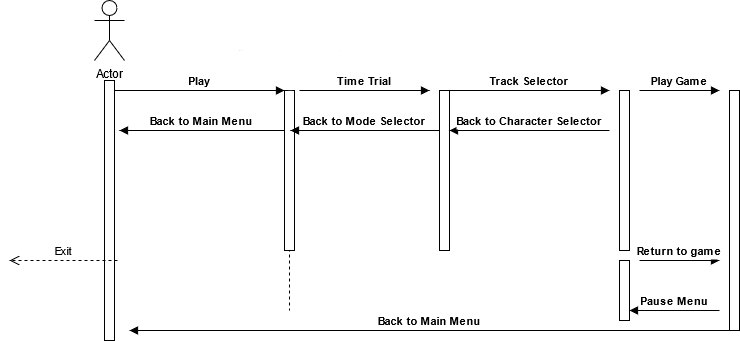
\includegraphics[width=\textwidth]{seq-diag}
	\caption{Diagrama de secuencias de ``Fastastic Roads''.}
	\label{fig:seq-diag}
\end{figure}

Entre los principales controladores esenciales se encuentra el controlador de carrera. Con ``RaceController'' se ha mantenido una relación directa con los \textit{checkpoints} para el control de los mismos y su correcto funcionamiento en el circuito. Los \textit{checkpoints} actúan a su vez tanto como puntos de control como línea de meta/salida. Éstos dependen entre sí para el debido transcurso de la carerra, permitiendo al vehículo bifurcaciones por distintos caminos donde pudiese haber puntos de control diferentes sin que esto afectara a la imposibilidad de finalizar una partida. 

\imagen{dia-obj-cpoints}{Diagrama de objetos del grafo de Checkpoints.}

\section{Diseño arquitectónico}

En ``Fastastic Roads'' se han aplicado algunos patrones de diseño a la hora de desarrollar el proyecto. Unity permite la implementación de patrones estandarizados, como el ``Modelo-Vista-Controlador''. A continuación, se procede a explicar los patrones implementados.

\subsection{Patrón estrategia}

Mediante la implementación de este patrón de comportamiento, se permite al algoritmo variar independientemente de los clientes que lo utilizan. Aplicado al proyecto, el control en el videojuego se abstrae, materializándose en distintas estrategias (para el control local de un jugador o multijugador, control en red, etc.) para poder incluir nuevas funcionalidades sin tener que modificar el código independientemente de quién los utiliza \cite{disman:estrat}.

\imagen{patron-estrategia}{Estructura del patrón de comportamiento estrategia.}

\subsection{Patrón método plantilla}

En el patrón de comportamiento método plantilla se define el esqueleto de un algoritmo en una operación, dejando algunos de los pasos para las subclases, para que éstas redefinan ciertos pasos del algoritmo sin cambiar su estructura general \cite{disman:metplan}.

En este proyecto, en el nivel abstracto de ``BaseInput'' se implementaban controles de bloqueo de las entradas comunes para todos los tipos de entradas y se delegaba a las subclases la captura de las entradas específicas. 

\imagen{patron-metodo-plantilla}{Estructura del patrón creacional método plantilla.}

\section{Diseño de interfaces}

Por último, respecto al diseño de interfaz se decidió por elementos simples.

Un buen diseño en una aplicación donde los componentes gráficos son notables y muy importantes de cara a la buena recepción del usuario como son los videojuegos, es muy importante. Sin embargo, en el desarrollo de un videojuego la interfaz, así como otros tantos elementos y funcionalidades del mismo, no se perfecciona dejándolo visualmente llamativo hasta que la aplicación está bastante avanzada, e incluso cercana a terminar.

No obstante, eso no implica que se tenga que descuidar, pues ha de ser accesible al usuario tanto en el juego final como en las fases de desarrollo. Por ello, se decidió la colocación de botones grandes en los distintos menús, fáciles de entender y eficientes con su función asignada.

\imagen{fastastic-design-menu}{A pesar de la carencia de colores y un diseño atractivo, un usuario medio es capaz de entenderlo fácilmente.}

A medida que el proyecto vaya creciendo y se vayan creando nuevas funcionalidades, los menús tendrán tipografías más agradables a la vista y los botones serán más llamativos que los actualmente asignados.

Respecto al juego en sí, es importante tener una buena implementación de las distintas funciones para poder disfrutar de él, pero con un mal diseño puede acabar aburriendo o cansando al usuario. Es por ello que este aspecto es más importante tenerlo trabajado desde un principio, por lo que el juego tiene escenarios altamente detallados y llamativos, así como unos diseños de vehículos que invitan al usuario a disfrutar de una conducción divertida con ellos.

\imagen{fastastic-design-track}{Los escenarios se han trabajado desde un principio, permitiendo mejoras a medida que se avanza con el proyecto.}

A ello se le añade un buen diseño de logotipo para la identificación del videojuego. Este logotipo tuvo una fase previa, y ahora mismo es el diseño final disponible con el cual se puede distinguir a ``Fastastic Roads''.

\imagen{fastastic-roads-logo}{El logotipo de ``Fastastic Roads'' apela a la estética industrial del videojuego.}
\apendice{Documentación técnica de programación}

\section{Introducción}

\section{Estructura de directorios}

\section{Manual del programador}

\section{Compilación, instalación y ejecución del proyecto}

\section{Pruebas del sistema}

\apendice{Documentación de usuario}

\section{Introducción}

En este apartado se recogen los requisitos mínimos para poder ejecutar la aplicación, así como los pasos a seguir para ejecutarla y un manual de uso de la misma.

\section{Requisitos de usuarios}

Los requisitos mínimos para ejecutar el videojuego, calculados en base a los mencionados por Unity en su página web, son los siguientes:

\begin{itemize}
\tightlist
	\item Procesador: cualquiera con arquitectura x86/x64 con soporte para set de instrucciones SSE2
	\item Memoria RAM: 4 gbs
	\item Tarjeta gráfica: cualquiera compatible con, al menos, DirectX 10
	\item Sistema operativo: Windows 7/8/10, solo en versión de 64 bits
	\item Ratón
	\item Teclado
\end{itemize}

De igual manera, se ha probado en diferentes PCs y los mínimos recomendados obtenidos, en base a esos PCs mencionados, son los siguientes:

\begin{itemize}
\tightlist
	\item Procesador: Intel i7-8750H/AMD FX 6350
	\item Memoria RAM: 8 GBs
	\item Tarjeta gráfica: Intel UHD Graphics 630 (media de entre 25 - 30 fps)
	\item Sistema operativo: Windows 7
	\item Espacio ocupado en SSD/HDD: 250 MBs aprox.
\end{itemize}

Tras haber probado con diferentes pantallas, la escalabilidad de la resolución con los elementos en pantalla no es automática, por lo que la resolución de pantalla recomendada para una correcta visualización es de 1920x1080.

\section{Instalación}

El videojuego se exporta directamente desde el mismo motor Unity como aplicación ejecutable. Gracias a ello no es necesaria la instalación del mismo, sino que se puede abrir haciendo doble \textit{click} directamente en el ejecutable con el nombre de ``Fastastic Roads''.

Es recomendable tener actualizada la tarjeta gráfica, así como los controladores correspondientes para que el videojuego pueda ser ejecutado.

\section{Manual del usuario}

El uso de la aplicación es muy sencillo. Se empezará ejecutando el juego, haciendo doble \textit{click} en el nombre de ``Fastastic Roads.exe'', correspondiente al ejecutable. Aparecerá el logo de Unity y, a continuación, aparecerá el menú principal.

\subsection{Menús}

Las pantallas por las que se mueve el usuario son menús. En estos menús habrá botones, en los cuales se puede pinchar con el botón izquierdo del ratón. Se procede a explicar las diferentes pantallas. Todos los menús tienen un botón para retroceder a la pantalla anterior en la esquina inferior izquierda.

\subsubsection{Menú principal}

Este menú es la pantalla principal del juego. Permite proceder a las distintas pantallas del juego, así como a salir de él. 
\begin{itemize}
\tightlist
	\item \textbf{Play}: permite trasladarse a la pantalla de selección de modo de juego.
	\item \textbf{Instructions}: muestra en pantalla las instrucciones de manejo de vehículo, para entender cómo jugar en una partida.
	\item \textbf{Credits}: aparecen las distintas personas involucradas en el proyecto y sus roles.
	\item \textbf{Exit}: permite salirse del videojuego, devolviendo al usuario a \textit{Windows}.
\end{itemize}

\imagen{fastastic-menu}{Menú principal de ``Fastastic Roads''.}

\subsubsection{Instrucciones}

Muestra las instrucciones de juego. El manejo de vehículo se puede realizar con las flechas del teclado, o bien con las teclas ``W'', ``A'', ``S'' y ``D'' siguiendo la misma posición que las flechas (flecha arriba - W, flecha izquierda - A, flecha abajo - S, flecha derecha - D). En caso de volcado de vehículo o cualquier otra situación que lo requiera, hay posibilidad de recolocar el vehículo en el último punto de control atravesado pulsando la tecla ``R''.

\imagen{fastastic-instructions}{Instrucciones para jugar.}

Para jugar correctamente, se explican los siguientes puntos:

\begin{itemize}
\tightlist
	\item El vehículo se mueve manteniendo pulsadas estas teclas. Si una tecla se pulsa pero no se mantiene, realizará un escaso movimiento. De igual manera, si una tecla se mantiene pulsada de manera constante, es probable que el usuario pierda el control del vehículo, por lo que tiene que hacer combinaciones de pulsaciones continuas y soltar las mismas teclas. Para jugadores menos experimentados, es aconsejable realizar toques cortos en las teclas para un mejor manejo en la partida
	\item Si el vehículo está parado y se pulsa la tecla correspondiente al giro a la izquierda o al giro a la derecha, éste se moverá sobre sí mismo hacia el lado correspondiente de la tecla pulsada.
	\item Si el vehículo está en movimiento sin acelerar y se pulsa la tecla correspondiente al giro a la izquierda o al giro a la derecha, éste se moverá siguiendo la inercia del mismo hacia el lado correspondiente de la tecla pulsada.
	\item Si se pulsa la tecla de aceleración sin combinar con ninguna tecla de giro, el vehículo se moverá en línea recta.
	\item Si se pulsa la tecla de deceleración, sin estar previamente el vehículo en movimiento y sin combinar con ninguna de giro, el vehículo se moverá marcha atrás en línea recta.
	\item Si se pulsa la tecla de deceleración estando previamente el vehículo en movimiento y sin combinar con ninguna de giro, el vehículo decelerará hasta detenerse. Si no se suelta la tecla de deceleración una vez el vehículo esté a punto de detenerse, iniciará la marcha atrás inmediatamente después.
	\item Si se pulsa la tecla de aceleración más una tecla de giro a la vez, el vehículo girará hacia la dirección deseada mientras avanza.
	\item Si se pulsa la tecla de deleración más una tecla de giro a la vez, el vehículo girará hacia la dirección deseada mientras avanza marcha atrás.
\end{itemize}

Para continuar hacia la partida, el usuario pulsará en ``\textit{Play}'' (``Jugar'').

\subsubsection{Selector de modo}

En esta pantalla se escoge entre los diferentes modos disponibles. En el caso de este proyecto, solo está disponible para seleccionar el modo contrarreloj (\textit{Time Trial}), con idea a futuro de integrar más modos, como el otro mostrado en rojo no seleccionable con el mensaje ``\textit{Coming soon}'' (``Disponible próximamente'').

\imagen{fastastic-modeselector}{Selector de modo de juego (solo disponible el modo a contrarreloj).}

El usuario pulsará en ``Time Trial'' para continuar a la partida.

\subsubsection{Selector de personaje}

Permite escoger entre los distintos personajes disponibles. Aunque aparezcan varios nombres, en este proyecto, independientemente de dónde se pulse, solo se podrá jugar con el personaje de ``Pilar Careaga''.

\imagen{fastastic-characterselector}{Selector de personaje (solo disponible el personaje de Pilar Careaga).}

Por ello, el usuario pulsará en cualquiera de los dos disponibles.

\subsubsection{Selector de circuito}

Antes de comenzar la partida, se escoge entre los distintos circuitos disponibles. De nuevo, solo hay un circuito disponible, por lo que independientemente de dónde se pulse llevará al mismo.

\imagen{fastastic-trackselector}{Selector de circuito para jugar (solo uno disponible).}

Por ello, el usuario escogerá cualquiera de los dos en pantalla.

\subsubsection{Partida contrarreloj}

Una vez comienza la partida, primero aparece una cuenta atrás en la cual el usuario no puede mover el vehículo hasta que haya terminado, donde aparecerá el mensaje ``\textit{Go!}'' (equivalente a ``¡Ya!'').

\imagen{fastastic-countdown}{Cuenta atrás antes de empezar la carrera.}

Con la cuenta atrás finalizada, el usuario puede empezar a moverse. Siguiendo las intrucciones anteriormente mencionadas, el usuario tiene que seguir por el circuito avanzando por la carretera atravesando los diferentes puntos de control hasta llegar a meta. 

\imagen{fastastic-checkpoint}{Los puntos de control se distinguen por su transparencia ligeramente traslúcida.}

Si el usuario se mueve en dirección contraria, los puntos de control que atraviese no serán válidos hasta que no llegue al que le corresponde atravesar inicialmente. Para que sea distinguible, hay diferentes señales con flechas indicativas en el escenario para orientar al jugador.

\imagen{fastastic-randomimage}{Las flechas indican por dónde debe ir el jugador.}

En la interfaz se puede observar un letrero de ``\textit{Lap}'', el cual indica el número de vuelta en el que se encuentra el usuario y el número total de vueltas de la carrera, así como otro letrero que indica el ``\textit{Lap time}'' o tiempo de vuelta, y el ``\textit{Best lap time}'' o mejor tiempo de vuelta.

\imagen{fastastic-twoways}{En algún punto del circuito puede haber bifurcaciones por las que circular.}

El usuario puede encontrarse durante el recorrido de la partida diferentes caminos por los que ir. Podrá escoger libremente entre cualquiera de ellos, donde la diferencia de cada uno la marca la dificultad de recorrido.

\imagen{fastastic-newlap}{Al pasar de nuevo por meta, se actualiza el número de vueltas y el mejor tiempo.}

Una vez atraviesa la meta después de haber pasado a través de todos los anteriores puntos de control, el contador de ``Tiempo por vuelta'' de restaura a cero, y si el tiempo ha sido mejor que el previo, se actualiza el contador de ``Mejor tiempo por vuelta''.

\imagen{fastastic-pausemenu}{Hay posibilidad de pausar la partida dándole a la tecla de Escape.}

En caso de que sea necesario, el videojuego se puede pausar pulsando la tecla de ``Escape'' en el teclado, permitiendo al usuario continuar el juego cuando se desee o, en caso contrario, abandonarlo, devolviendo al usuario de esta manera al menú principal.

\imagen{fastastic-endgame}{Al finalizar, se bloquea el manejo del vehículo y se salta a la pantalla de estadísticas.}

Una vez se completen todas las vueltas, el vehículo bloquea su control impidiendo moverlo con el teclado, y devolviendo al usuario a la pantalla de estadísticas.

\subsubsection{Créditos}

Para finalizar, aquí se muestra una descripción del proyecto y los distintos participantes que han colaborado en él.

\imagen{fastastic-credits}{En la pantalla de créditos aparecen los participantes en el desarrollo del proyecto.}


\bibliographystyle{plain}
\bibliography{bibliografiaAnexos}

\end{document}
